\documentclass[border=4pt]{standalone}
\usepackage{fontspec}
\usepackage{amsmath}
\usepackage{unicode-math}
\setmainfont{Latin Modern Roman}
\setmathfont{Latin Modern Math}
\usepackage{pgfplots}
\usepackage{pgfplotstable}
\pgfplotsset{compat=1.18}
\usepackage{tkz-euclide}
\usetikzlibrary{arrows.meta,calc,angles,quotes,patterns,3d,backgrounds}
\definecolor{ink}{HTML}{123428}
\definecolor{asy}{HTML}{475569}
\definecolor{mint}{HTML}{86e0bd}
\tikzset{asym/.style={asy, line width=0.9pt, dash pattern=on 5pt off 3.5pt},
         guide/.style={gray!70, line width=0.6pt, densely dotted},
         dot/.style={circle, inner sep=0pt, minimum size=5pt, draw=white, line width=0.5pt},
         odot/.style={circle, inner sep=0pt, minimum size=5.5pt, fill=white, line width=1pt},
         lab/.style={font=\footnotesize, inner sep=1.5pt, text=ink}}
\begin{document}
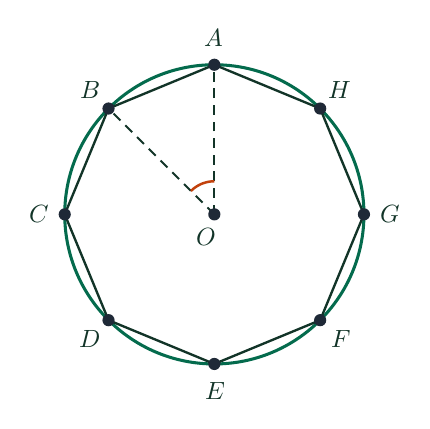
\begin{tikzpicture}
\draw[color={rgb,255:red,4;green,107;blue,77}, line width=1.1pt] (0,0) circle (1.900);
\draw[ink, line width=0.85pt] (0.000,1.900) -- (-1.344,1.344);
\draw[ink, line width=0.85pt] (-1.344,1.344) -- (-1.900,0.000);
\draw[ink, line width=0.85pt] (-1.900,0.000) -- (-1.344,-1.344);
\draw[ink, line width=0.85pt] (-1.344,-1.344) -- (-0.000,-1.900);
\draw[ink, line width=0.85pt] (-0.000,-1.900) -- (1.344,-1.344);
\draw[ink, line width=0.85pt] (1.344,-1.344) -- (1.900,-0.000);
\draw[ink, line width=0.85pt] (1.900,-0.000) -- (1.344,1.344);
\draw[ink, line width=0.85pt] (1.344,1.344) -- (0.000,1.900);
\draw[ink, line width=0.7pt, dash pattern=on 3.5pt off 2.5pt] (0.000,0.000) -- (0.000,1.900);
\draw[ink, line width=0.7pt, dash pattern=on 3.5pt off 2.5pt] (0.000,0.000) -- (-1.344,1.344);
\draw[color={rgb,255:red,194;green,65;blue,12}, line width=0.9pt] (0.000,0.420) -- (-0.016,0.420) -- (-0.033,0.419) -- (-0.049,0.417) -- (-0.066,0.415) -- (-0.082,0.412) -- (-0.098,0.408) -- (-0.114,0.404) -- (-0.130,0.399) -- (-0.145,0.394) -- (-0.161,0.388) -- (-0.176,0.381) -- (-0.191,0.374) -- (-0.205,0.366) -- (-0.219,0.358) -- (-0.233,0.349) -- (-0.247,0.340) -- (-0.260,0.330) -- (-0.273,0.319) -- (-0.285,0.308) -- (-0.297,0.297);
\fill[color={rgb,255:red,31;green,41;blue,55}] (0.000,1.900) circle (2.2pt);
\fill[color={rgb,255:red,31;green,41;blue,55}] (-1.344,1.344) circle (2.2pt);
\fill[color={rgb,255:red,31;green,41;blue,55}] (-1.900,0.000) circle (2.2pt);
\fill[color={rgb,255:red,31;green,41;blue,55}] (-1.344,-1.344) circle (2.2pt);
\fill[color={rgb,255:red,31;green,41;blue,55}] (-0.000,-1.900) circle (2.2pt);
\fill[color={rgb,255:red,31;green,41;blue,55}] (1.344,-1.344) circle (2.2pt);
\fill[color={rgb,255:red,31;green,41;blue,55}] (1.900,-0.000) circle (2.2pt);
\fill[color={rgb,255:red,31;green,41;blue,55}] (1.344,1.344) circle (2.2pt);
\fill[color={rgb,255:red,31;green,41;blue,55}] (0.000,0.000) circle (2.2pt);
\node[font=\small, text=ink, inner sep=0.5pt] at (0.000,2.240) {$A$};
\node[font=\small, text=ink, inner sep=0.5pt] at (-1.584,1.584) {$B$};
\node[font=\small, text=ink, inner sep=0.5pt] at (-2.240,0.000) {$C$};
\node[font=\small, text=ink, inner sep=0.5pt] at (-1.584,-1.584) {$D$};
\node[font=\small, text=ink, inner sep=0.5pt] at (-0.000,-2.240) {$E$};
\node[font=\small, text=ink, inner sep=0.5pt] at (1.584,-1.584) {$F$};
\node[font=\small, text=ink, inner sep=0.5pt] at (2.240,-0.000) {$G$};
\node[font=\small, text=ink, inner sep=0.5pt] at (1.584,1.584) {$H$};
\node[font=\small, text=ink, inner sep=0.5pt] at (-0.103,-0.282) {$O$};
\end{tikzpicture}
\end{document}
